\documentclass[twoside]{book}

% Packages required by doxygen
\usepackage{fixltx2e}
\usepackage{calc}
\usepackage{doxygen}
\usepackage[export]{adjustbox} % also loads graphicx
\usepackage{graphicx}
\usepackage[utf8]{inputenc}
\usepackage{makeidx}
\usepackage{multicol}
\usepackage{multirow}
\PassOptionsToPackage{warn}{textcomp}
\usepackage{textcomp}
\usepackage[nointegrals]{wasysym}
\usepackage[table]{xcolor}

% Font selection
\usepackage[T1]{fontenc}
\usepackage[scaled=.90]{helvet}
\usepackage{courier}
\usepackage{amssymb}
\usepackage{sectsty}
\renewcommand{\familydefault}{\sfdefault}
\allsectionsfont{%
  \fontseries{bc}\selectfont%
  \color{darkgray}%
}
\renewcommand{\DoxyLabelFont}{%
  \fontseries{bc}\selectfont%
  \color{darkgray}%
}
\newcommand{\+}{\discretionary{\mbox{\scriptsize$\hookleftarrow$}}{}{}}

% Page & text layout
\usepackage{geometry}
\geometry{%
  a4paper,%
  top=2.5cm,%
  bottom=2.5cm,%
  left=2.5cm,%
  right=2.5cm%
}
\tolerance=750
\hfuzz=15pt
\hbadness=750
\setlength{\emergencystretch}{15pt}
\setlength{\parindent}{0cm}
\setlength{\parskip}{3ex plus 2ex minus 2ex}
\makeatletter
\renewcommand{\paragraph}{%
  \@startsection{paragraph}{4}{0ex}{-1.0ex}{1.0ex}{%
    \normalfont\normalsize\bfseries\SS@parafont%
  }%
}
\renewcommand{\subparagraph}{%
  \@startsection{subparagraph}{5}{0ex}{-1.0ex}{1.0ex}{%
    \normalfont\normalsize\bfseries\SS@subparafont%
  }%
}
\makeatother

% Headers & footers
\usepackage{fancyhdr}
\pagestyle{fancyplain}
\fancyhead[LE]{\fancyplain{}{\bfseries\thepage}}
\fancyhead[CE]{\fancyplain{}{}}
\fancyhead[RE]{\fancyplain{}{\bfseries\leftmark}}
\fancyhead[LO]{\fancyplain{}{\bfseries\rightmark}}
\fancyhead[CO]{\fancyplain{}{}}
\fancyhead[RO]{\fancyplain{}{\bfseries\thepage}}
\fancyfoot[LE]{\fancyplain{}{}}
\fancyfoot[CE]{\fancyplain{}{}}
\fancyfoot[RE]{\fancyplain{}{\bfseries\scriptsize Generated by Doxygen }}
\fancyfoot[LO]{\fancyplain{}{\bfseries\scriptsize Generated by Doxygen }}
\fancyfoot[CO]{\fancyplain{}{}}
\fancyfoot[RO]{\fancyplain{}{}}
\renewcommand{\footrulewidth}{0.4pt}
\renewcommand{\chaptermark}[1]{%
  \markboth{#1}{}%
}
\renewcommand{\sectionmark}[1]{%
  \markright{\thesection\ #1}%
}

% Indices & bibliography
\usepackage{natbib}
\usepackage[titles]{tocloft}
\setcounter{tocdepth}{3}
\setcounter{secnumdepth}{5}
\makeindex

% Hyperlinks (required, but should be loaded last)
\usepackage{ifpdf}
\ifpdf
  \usepackage[pdftex,pagebackref=true]{hyperref}
\else
  \usepackage[ps2pdf,pagebackref=true]{hyperref}
\fi
\hypersetup{%
  colorlinks=true,%
  linkcolor=blue,%
  citecolor=blue,%
  unicode%
}

% Custom commands
\newcommand{\clearemptydoublepage}{%
  \newpage{\pagestyle{empty}\cleardoublepage}%
}

\usepackage{caption}
\captionsetup{labelsep=space,justification=centering,font={bf},singlelinecheck=off,skip=4pt,position=top}

%===== C O N T E N T S =====

\begin{document}

% Titlepage & ToC
\hypersetup{pageanchor=false,
             bookmarksnumbered=true,
             pdfencoding=unicode
            }
\pagenumbering{alph}
\begin{titlepage}
\vspace*{7cm}
\begin{center}%
{\Large My Project }\\
\vspace*{1cm}
{\large Generated by Doxygen 1.8.13}\\
\end{center}
\end{titlepage}
\clearemptydoublepage
\pagenumbering{roman}
\tableofcontents
\clearemptydoublepage
\pagenumbering{arabic}
\hypersetup{pageanchor=true}

%--- Begin generated contents ---
\chapter{Hierarchical Index}
\section{Class Hierarchy}
This inheritance list is sorted roughly, but not completely, alphabetically\+:\begin{DoxyCompactList}
\item \contentsline{section}{Alarm}{\pageref{class_alarm}}{}
\item \contentsline{section}{Data\+Logger}{\pageref{class_data_logger}}{}
\item \contentsline{section}{Sd\+Csd}{\pageref{struct_sd_csd}}{}
\item spi\+\_\+bus\begin{DoxyCompactList}
\item \contentsline{section}{due\+:\+:spi\+\_\+bus\+\_\+due}{\pageref{classdue_1_1spi__bus__due}}{}
\end{DoxyCompactList}
\item Store\begin{DoxyCompactList}
\item \contentsline{section}{Sd\+Spi}{\pageref{class_sd_spi}}{}
\end{DoxyCompactList}
\end{DoxyCompactList}

\chapter{Class Index}
\section{Class List}
Here are the classes, structs, unions and interfaces with brief descriptions\+:\begin{DoxyCompactList}
\item\contentsline{section}{\hyperlink{class_alarm}{Alarm} }{\pageref{class_alarm}}{}
\item\contentsline{section}{\hyperlink{class_data_logger}{Data\+Logger} }{\pageref{class_data_logger}}{}
\item\contentsline{section}{\hyperlink{struct_sd_csd}{Sd\+Csd} \\*SD Card-\/\+Specific Data structure }{\pageref{struct_sd_csd}}{}
\item\contentsline{section}{\hyperlink{class_sd_spi}{Sd\+Spi} \\*Provides a SD S\+PI Block Storage Provider }{\pageref{class_sd_spi}}{}
\item\contentsline{section}{\hyperlink{classdue_1_1spi__bus__due}{due\+::spi\+\_\+bus\+\_\+due} \\*Due / sam3x8e native S\+PI bus }{\pageref{classdue_1_1spi__bus__due}}{}
\end{DoxyCompactList}

\chapter{File Index}
\section{File List}
Here is a list of all documented files with brief descriptions\+:\begin{DoxyCompactList}
\item\contentsline{section}{\hyperlink{alarm_8cc}{alarm.\+cc} \\*The definitions of the alarm functionality of G\+A\+S-\/01 }{\pageref{alarm_8cc}}{}
\item\contentsline{section}{\hyperlink{alarm_8hh}{alarm.\+hh} \\*The declarations of the class \hyperlink{class_alarm}{Alarm} of G\+A\+S-\/01 }{\pageref{alarm_8hh}}{}
\item\contentsline{section}{\hyperlink{data-logger_8cc}{data-\/logger.\+cc} \\*Logs sensor data to the sd card }{\pageref{data-logger_8cc}}{}
\item\contentsline{section}{\hyperlink{data-logger_8hh}{data-\/logger.\+hh} \\*Logs sensor data to the sd card }{\pageref{data-logger_8hh}}{}
\item\contentsline{section}{\hyperlink{hwlib-due-spi_8hh}{hwlib-\/due-\/spi.\+hh} \\*Due / sam3x8e native S\+PI }{\pageref{hwlib-due-spi_8hh}}{}
\item\contentsline{section}{\hyperlink{libc-stub_8cc}{libc-\/stub.\+cc} \\*Libc stub code }{\pageref{libc-stub_8cc}}{}
\item\contentsline{section}{\hyperlink{main_8cc}{main.\+cc} \\*G\+AS module main }{\pageref{main_8cc}}{}
\item\contentsline{section}{\hyperlink{sd-spi_8cc}{sd-\/spi.\+cc} \\*SD S\+PI Store provider }{\pageref{sd-spi_8cc}}{}
\item\contentsline{section}{\hyperlink{sd-spi_8hh}{sd-\/spi.\+hh} \\*SD S\+PI Store provider }{\pageref{sd-spi_8hh}}{}
\item\contentsline{section}{{\bfseries wrap-\/hwlib.\+hh} }{\pageref{wrap-hwlib_8hh}}{}
\end{DoxyCompactList}

\chapter{Class Documentation}
\hypertarget{class_alarm}{}\section{Alarm Class Reference}
\label{class_alarm}\index{Alarm@{Alarm}}
\subsection*{Public Member Functions}
\begin{DoxyCompactItemize}
\item 
\mbox{\Hypertarget{class_alarm_af1e2f02eb5f9d8dbc6d8889792cad21b}\label{class_alarm_af1e2f02eb5f9d8dbc6d8889792cad21b}} 
\hyperlink{class_alarm_af1e2f02eb5f9d8dbc6d8889792cad21b}{Alarm} (float gas\+Value\+Threshold, hwlib\+::pin\+\_\+out \&alarm\+Led)
\begin{DoxyCompactList}\small\item\em Constructor for \hyperlink{class_alarm}{Alarm} Initializes gas\+Value\+Threshold and alarm\+Led. \end{DoxyCompactList}\item 
void \hyperlink{class_alarm_a9e63742ac82c56fb1da7d37e8fcf812c}{check\+Gas\+Value} (float gas\+Value)
\begin{DoxyCompactList}\small\item\em Check if gas value is above the threshold then trigger the alarm Take the gas value and call trigger\+Alarm() when it\textquotesingle{}s above the threshold or disable\+Alarm() when it\textquotesingle{}s below said threshold. \end{DoxyCompactList}\end{DoxyCompactItemize}


\subsection{Member Function Documentation}
\mbox{\Hypertarget{class_alarm_a9e63742ac82c56fb1da7d37e8fcf812c}\label{class_alarm_a9e63742ac82c56fb1da7d37e8fcf812c}} 
\index{Alarm@{Alarm}!check\+Gas\+Value@{check\+Gas\+Value}}
\index{check\+Gas\+Value@{check\+Gas\+Value}!Alarm@{Alarm}}
\subsubsection{\texorpdfstring{check\+Gas\+Value()}{checkGasValue()}}
{\footnotesize\ttfamily void Alarm\+::check\+Gas\+Value (\begin{DoxyParamCaption}\item[{float}]{gas\+Value }\end{DoxyParamCaption})}



Check if gas value is above the threshold then trigger the alarm Take the gas value and call trigger\+Alarm() when it\textquotesingle{}s above the threshold or disable\+Alarm() when it\textquotesingle{}s below said threshold. 


\begin{DoxyParams}{Parameters}
{\em gas\+Value} & the gas value \\
\hline
\end{DoxyParams}


The documentation for this class was generated from the following files\+:\begin{DoxyCompactItemize}
\item 
C\+:/\+H\+U (school)/jaar2.\+2/(4) R2\+D2/\+R2\+D2-\/2017/modules/\+G\+A\+S/src/\hyperlink{alarm_8hh}{alarm.\+hh}\item 
C\+:/\+H\+U (school)/jaar2.\+2/(4) R2\+D2/\+R2\+D2-\/2017/modules/\+G\+A\+S/src/\hyperlink{alarm_8cc}{alarm.\+cc}\end{DoxyCompactItemize}

\hypertarget{class_data_logger}{}\section{Data\+Logger Class Reference}
\label{class_data_logger}\index{Data\+Logger@{Data\+Logger}}
\subsection*{Public Member Functions}
\begin{DoxyCompactItemize}
\item 
void \hyperlink{class_data_logger_a6bc493c434d247169fdcca030eed7451}{write\+Value} (float value)
\begin{DoxyCompactList}\small\item\em Logs a value onto the sd card. \end{DoxyCompactList}\item 
\hyperlink{class_data_logger_a4e0a4ccbd4b3ecd0d05a57bc8f26dc24}{Data\+Logger} (\hyperlink{class_sd_spi}{Sd\+Spi} \&sd)
\begin{DoxyCompactList}\small\item\em Creates a data logger object to write sensor data to a sd card. \end{DoxyCompactList}\end{DoxyCompactItemize}


\subsection{Constructor \& Destructor Documentation}
\mbox{\Hypertarget{class_data_logger_a4e0a4ccbd4b3ecd0d05a57bc8f26dc24}\label{class_data_logger_a4e0a4ccbd4b3ecd0d05a57bc8f26dc24}} 
\index{Data\+Logger@{Data\+Logger}!Data\+Logger@{Data\+Logger}}
\index{Data\+Logger@{Data\+Logger}!Data\+Logger@{Data\+Logger}}
\subsubsection{\texorpdfstring{Data\+Logger()}{DataLogger()}}
{\footnotesize\ttfamily Data\+Logger\+::\+Data\+Logger (\begin{DoxyParamCaption}\item[{\hyperlink{class_sd_spi}{Sd\+Spi} \&}]{sd }\end{DoxyParamCaption})}



Creates a data logger object to write sensor data to a sd card. 


\begin{DoxyParams}{Parameters}
{\em sd} & The SD card to write the data to \\
\hline
\end{DoxyParams}


\subsection{Member Function Documentation}
\mbox{\Hypertarget{class_data_logger_a6bc493c434d247169fdcca030eed7451}\label{class_data_logger_a6bc493c434d247169fdcca030eed7451}} 
\index{Data\+Logger@{Data\+Logger}!write\+Value@{write\+Value}}
\index{write\+Value@{write\+Value}!Data\+Logger@{Data\+Logger}}
\subsubsection{\texorpdfstring{write\+Value()}{writeValue()}}
{\footnotesize\ttfamily void Data\+Logger\+::write\+Value (\begin{DoxyParamCaption}\item[{float}]{value }\end{DoxyParamCaption})}



Logs a value onto the sd card. 


\begin{DoxyParams}{Parameters}
{\em The} & value to log \\
\hline
\end{DoxyParams}


The documentation for this class was generated from the following files\+:\begin{DoxyCompactItemize}
\item 
\hyperlink{data-logger_8hh}{data-\/logger.\+hh}\item 
\hyperlink{data-logger_8cc}{data-\/logger.\+cc}\end{DoxyCompactItemize}

\hypertarget{struct_sd_csd}{}\section{Sd\+Csd Struct Reference}
\label{struct_sd_csd}\index{Sd\+Csd@{Sd\+Csd}}


SD Card-\/\+Specific Data structure.  


\subsection*{Public Attributes}
\begin{DoxyCompactItemize}
\item 
\mbox{\Hypertarget{struct_sd_csd_a38887142a7b15bf54b2082092f8c8784}\label{struct_sd_csd_a38887142a7b15bf54b2082092f8c8784}} 
uint8\+\_\+t {\bfseries version}\+: 2
\item 
\mbox{\Hypertarget{struct_sd_csd_af91da518406dad96dfd13386fd47f9ee}\label{struct_sd_csd_af91da518406dad96dfd13386fd47f9ee}} 
uint8\+\_\+t {\bfseries \+\_\+reserved1}\+: 6
\item 
\mbox{\Hypertarget{struct_sd_csd_ae3a34a8bbcf79cad9d78674d1c850bc8}\label{struct_sd_csd_ae3a34a8bbcf79cad9d78674d1c850bc8}} 
uint8\+\_\+t {\bfseries taac}\+: 8
\item 
\mbox{\Hypertarget{struct_sd_csd_ad99b4989c57a7ce428fbc3a809bd28c9}\label{struct_sd_csd_ad99b4989c57a7ce428fbc3a809bd28c9}} 
uint8\+\_\+t {\bfseries nsac}\+: 8
\item 
\mbox{\Hypertarget{struct_sd_csd_a41a489d630da13299ed6379c7b19e896}\label{struct_sd_csd_a41a489d630da13299ed6379c7b19e896}} 
uint8\+\_\+t {\bfseries tran\+Speed}\+: 8
\item 
\mbox{\Hypertarget{struct_sd_csd_a004ba330fd26d4da867252d6b2c09bfa}\label{struct_sd_csd_a004ba330fd26d4da867252d6b2c09bfa}} 
uint16\+\_\+t {\bfseries ccc}\+: 12
\item 
\mbox{\Hypertarget{struct_sd_csd_abcd97c7dd77397f932ac7d0af1c09891}\label{struct_sd_csd_abcd97c7dd77397f932ac7d0af1c09891}} 
uint8\+\_\+t {\bfseries read\+Bl\+Len}\+: 4
\item 
\mbox{\Hypertarget{struct_sd_csd_ac8a797b25ef8f94bca62f9adea5b4bf9}\label{struct_sd_csd_ac8a797b25ef8f94bca62f9adea5b4bf9}} 
uint8\+\_\+t {\bfseries read\+Bl\+Partial}\+: 1
\item 
\mbox{\Hypertarget{struct_sd_csd_a36d41621e9f3351be6ca8f5f6f8ab9c3}\label{struct_sd_csd_a36d41621e9f3351be6ca8f5f6f8ab9c3}} 
uint8\+\_\+t {\bfseries write\+Blk\+Misalign}\+: 1
\item 
\mbox{\Hypertarget{struct_sd_csd_ae9184f5bc32d7d798fb5c4797ff9fd87}\label{struct_sd_csd_ae9184f5bc32d7d798fb5c4797ff9fd87}} 
uint8\+\_\+t {\bfseries read\+Blk\+Misalign}\+: 1
\item 
\mbox{\Hypertarget{struct_sd_csd_a9c84095363b4c7fce7f914635324c643}\label{struct_sd_csd_a9c84095363b4c7fce7f914635324c643}} 
uint8\+\_\+t {\bfseries dsr\+Imp}\+: 1
\item 
\mbox{\Hypertarget{struct_sd_csd_a7c8f5992764703e08715d878e2b208f6}\label{struct_sd_csd_a7c8f5992764703e08715d878e2b208f6}} 
uint8\+\_\+t {\bfseries \+\_\+reserved2}\+: 6
\item 
\mbox{\Hypertarget{struct_sd_csd_ac8b7bf34f6fa0a2ce40545f5103cddeb}\label{struct_sd_csd_ac8b7bf34f6fa0a2ce40545f5103cddeb}} 
uint32\+\_\+t {\bfseries c\+Size}\+: 22
\item 
\mbox{\Hypertarget{struct_sd_csd_a63e30705b0af20cf51c9a9bd4cb15847}\label{struct_sd_csd_a63e30705b0af20cf51c9a9bd4cb15847}} 
uint8\+\_\+t {\bfseries \+\_\+reserved3}\+: 1
\item 
\mbox{\Hypertarget{struct_sd_csd_a73510dd43539d7bd227930eb653a0dca}\label{struct_sd_csd_a73510dd43539d7bd227930eb653a0dca}} 
uint8\+\_\+t {\bfseries erase\+Blk\+En}\+: 1
\item 
\mbox{\Hypertarget{struct_sd_csd_a31aa159eb93b279a953bddcecdc02d30}\label{struct_sd_csd_a31aa159eb93b279a953bddcecdc02d30}} 
uint8\+\_\+t {\bfseries sector\+Size}\+: 7
\item 
\mbox{\Hypertarget{struct_sd_csd_acfe668169ddf0b15ba4f58ccd676e459}\label{struct_sd_csd_acfe668169ddf0b15ba4f58ccd676e459}} 
uint8\+\_\+t {\bfseries wp\+Grp\+Size}\+: 7
\item 
\mbox{\Hypertarget{struct_sd_csd_a95dca80e995753f24e0ec5a3350ee4cb}\label{struct_sd_csd_a95dca80e995753f24e0ec5a3350ee4cb}} 
uint8\+\_\+t {\bfseries wp\+Grp\+Enable}\+: 1
\item 
\mbox{\Hypertarget{struct_sd_csd_aafde4fab15de6f48778eb8b920c8cc41}\label{struct_sd_csd_aafde4fab15de6f48778eb8b920c8cc41}} 
uint8\+\_\+t {\bfseries \+\_\+reserved4}\+: 2
\item 
\mbox{\Hypertarget{struct_sd_csd_aa4e28881f38c3a19073bacfb2abbd614}\label{struct_sd_csd_aa4e28881f38c3a19073bacfb2abbd614}} 
uint8\+\_\+t {\bfseries r2w\+Factor}\+: 3
\item 
\mbox{\Hypertarget{struct_sd_csd_a9676463e5bdcf447e0501c79581f28ed}\label{struct_sd_csd_a9676463e5bdcf447e0501c79581f28ed}} 
uint8\+\_\+t {\bfseries write\+Bl\+Len}\+: 4
\item 
\mbox{\Hypertarget{struct_sd_csd_a2ec228b74e44685c87c7f8fc5a1527e8}\label{struct_sd_csd_a2ec228b74e44685c87c7f8fc5a1527e8}} 
uint8\+\_\+t {\bfseries write\+Bl\+Partial}\+: 1
\item 
\mbox{\Hypertarget{struct_sd_csd_adfc80945cd5e7b5785a45349b1f2036c}\label{struct_sd_csd_adfc80945cd5e7b5785a45349b1f2036c}} 
uint8\+\_\+t {\bfseries \+\_\+reserved5}\+: 5
\item 
\mbox{\Hypertarget{struct_sd_csd_ada3bdf7a3821b09329407a7c872bcdb2}\label{struct_sd_csd_ada3bdf7a3821b09329407a7c872bcdb2}} 
uint8\+\_\+t {\bfseries file\+Format\+Grp}\+: 1
\item 
\mbox{\Hypertarget{struct_sd_csd_a339fdc61e0628a61d83fd75e8e383cd8}\label{struct_sd_csd_a339fdc61e0628a61d83fd75e8e383cd8}} 
uint8\+\_\+t {\bfseries copy}\+: 1
\item 
\mbox{\Hypertarget{struct_sd_csd_a4f833463f25d4e572bff2922061c5bd4}\label{struct_sd_csd_a4f833463f25d4e572bff2922061c5bd4}} 
uint8\+\_\+t {\bfseries perm\+Write\+Protect}\+: 1
\item 
\mbox{\Hypertarget{struct_sd_csd_a544fbf58619407e50c16e725ea93a858}\label{struct_sd_csd_a544fbf58619407e50c16e725ea93a858}} 
uint8\+\_\+t {\bfseries tmp\+Write\+Protect}\+: 1
\item 
\mbox{\Hypertarget{struct_sd_csd_abd1d77966aa79bb40691ed2b41d6d5e3}\label{struct_sd_csd_abd1d77966aa79bb40691ed2b41d6d5e3}} 
uint8\+\_\+t {\bfseries file\+Format}\+: 2
\item 
\mbox{\Hypertarget{struct_sd_csd_aff4c075422b25c3b28ee8b9dc7908f14}\label{struct_sd_csd_aff4c075422b25c3b28ee8b9dc7908f14}} 
uint8\+\_\+t {\bfseries \+\_\+reserved6}\+: 2
\item 
\mbox{\Hypertarget{struct_sd_csd_ab4f8645c6177af04bb5fc38a7d23fac3}\label{struct_sd_csd_ab4f8645c6177af04bb5fc38a7d23fac3}} 
uint8\+\_\+t {\bfseries crc7}\+: 7
\item 
\mbox{\Hypertarget{struct_sd_csd_a9aa65519352646ed14338ab0cc064362}\label{struct_sd_csd_a9aa65519352646ed14338ab0cc064362}} 
uint8\+\_\+t {\bfseries \+\_\+end\+Bit}\+: 1
\end{DoxyCompactItemize}


\subsection{Detailed Description}
SD Card-\/\+Specific Data structure. 

Fields are named as in the simplified SD spec.

Note\+: This bitfield struct serves only as documentation in this file. It isn\textquotesingle{}t used in code. 

The documentation for this struct was generated from the following file\+:\begin{DoxyCompactItemize}
\item 
\hyperlink{sd-spi_8cc}{sd-\/spi.\+cc}\end{DoxyCompactItemize}

\hypertarget{class_sd_spi}{}\section{Sd\+Spi Class Reference}
\label{class_sd_spi}\index{Sd\+Spi@{Sd\+Spi}}


Provides a SD S\+PI Block Storage Provider.  




{\ttfamily \#include $<$sd-\/spi.\+hh$>$}

Inheritance diagram for Sd\+Spi\+:\begin{figure}[H]
\begin{center}
\leavevmode
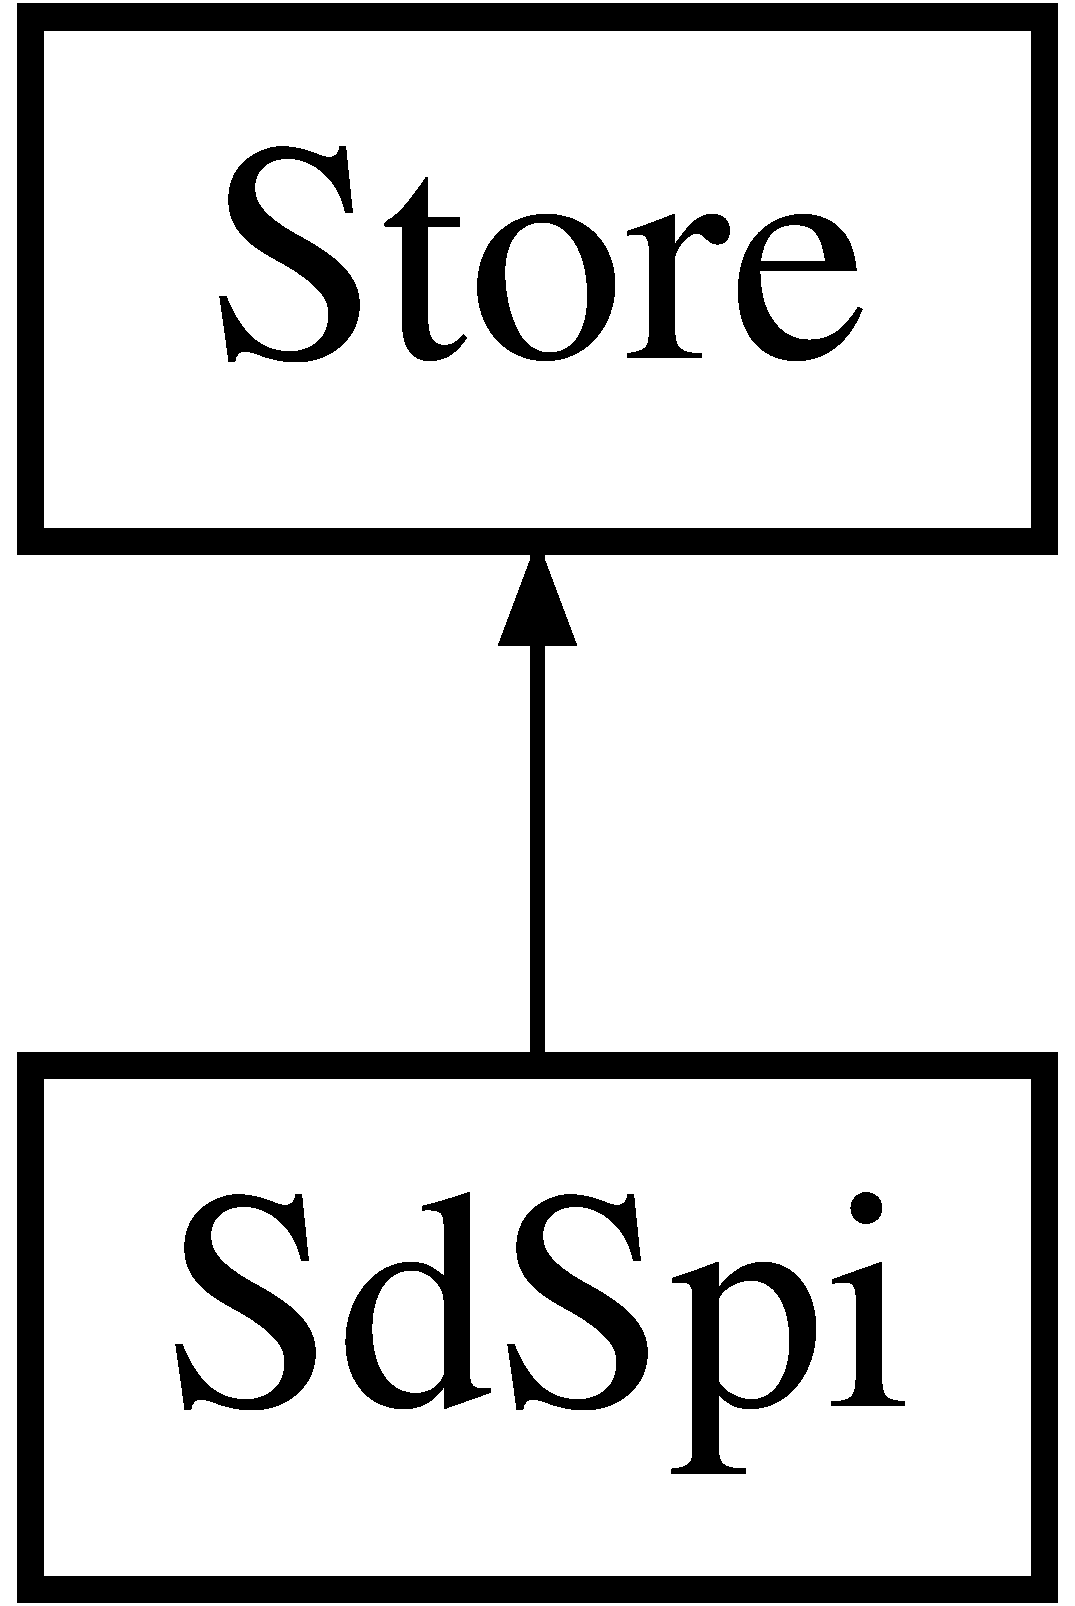
\includegraphics[height=2.000000cm]{class_sd_spi}
\end{center}
\end{figure}
\subsection*{Public Member Functions}
\begin{DoxyCompactItemize}
\item 
Mu\+Store\+::\+Store\+Error \hyperlink{class_sd_spi_a4120c7d7ccaeba5b2726f0fca6a97e9c}{seek} (size\+\_\+t lba)
\begin{DoxyCompactList}\small\item\em Seeks to a position within the sd card. \end{DoxyCompactList}\item 
Mu\+Store\+::\+Store\+Error \hyperlink{class_sd_spi_a90ee59c74ce983406c769b76c0083aa4}{read} (void $\ast$buffer)
\begin{DoxyCompactList}\small\item\em Reads a block from the sd card into a buffer. \end{DoxyCompactList}\item 
Mu\+Store\+::\+Store\+Error \hyperlink{class_sd_spi_ab3b314f23176ef7ed1197fb73d34f86f}{write} (const void $\ast$buffer)
\begin{DoxyCompactList}\small\item\em Writes a block from a buffer to the sd card. \end{DoxyCompactList}\item 
\hyperlink{class_sd_spi_a5a813ec0573cab136e4248787a46541a}{Sd\+Spi} (hwlib\+::pin\+\_\+out \&cs, hwlib\+::spi\+\_\+bus \&bus)
\begin{DoxyCompactList}\small\item\em Creates a SD S\+PI Block Provider. \end{DoxyCompactList}\end{DoxyCompactItemize}
\subsection*{Static Public Attributes}
\begin{DoxyCompactItemize}
\item 
static constexpr size\+\_\+t \hyperlink{class_sd_spi_a2eedef2fa6ec9844743e4e0de6f03261}{tmp\+Block\+Size} = 512
\end{DoxyCompactItemize}


\subsection{Detailed Description}
Provides a SD S\+PI Block Storage Provider. 

\subsection{Constructor \& Destructor Documentation}
\mbox{\Hypertarget{class_sd_spi_a5a813ec0573cab136e4248787a46541a}\label{class_sd_spi_a5a813ec0573cab136e4248787a46541a}} 
\index{Sd\+Spi@{Sd\+Spi}!Sd\+Spi@{Sd\+Spi}}
\index{Sd\+Spi@{Sd\+Spi}!Sd\+Spi@{Sd\+Spi}}
\subsubsection{\texorpdfstring{Sd\+Spi()}{SdSpi()}}
{\footnotesize\ttfamily Sd\+Spi\+::\+Sd\+Spi (\begin{DoxyParamCaption}\item[{hwlib\+::pin\+\_\+out \&}]{cs,  }\item[{hwlib\+::spi\+\_\+bus \&}]{bus }\end{DoxyParamCaption})}



Creates a SD S\+PI Block Provider. 


\begin{DoxyParams}{Parameters}
{\em cs} & The CS pin the sd card reader is connected to \\
\hline
{\em bus} & The spi bus the sd card reader is connected to \\
\hline
\end{DoxyParams}


\subsection{Member Function Documentation}
\mbox{\Hypertarget{class_sd_spi_a90ee59c74ce983406c769b76c0083aa4}\label{class_sd_spi_a90ee59c74ce983406c769b76c0083aa4}} 
\index{Sd\+Spi@{Sd\+Spi}!read@{read}}
\index{read@{read}!Sd\+Spi@{Sd\+Spi}}
\subsubsection{\texorpdfstring{read()}{read()}}
{\footnotesize\ttfamily Store\+Error Sd\+Spi\+::read (\begin{DoxyParamCaption}\item[{void $\ast$}]{buffer }\end{DoxyParamCaption})}



Reads a block from the sd card into a buffer. 


\begin{DoxyParams}{Parameters}
{\em buffer} & The buffer to read the block into \\
\hline
\end{DoxyParams}
\begin{DoxyReturn}{Returns}
Returns the status code if the reading was successful or not 
\end{DoxyReturn}
\mbox{\Hypertarget{class_sd_spi_a4120c7d7ccaeba5b2726f0fca6a97e9c}\label{class_sd_spi_a4120c7d7ccaeba5b2726f0fca6a97e9c}} 
\index{Sd\+Spi@{Sd\+Spi}!seek@{seek}}
\index{seek@{seek}!Sd\+Spi@{Sd\+Spi}}
\subsubsection{\texorpdfstring{seek()}{seek()}}
{\footnotesize\ttfamily Store\+Error Sd\+Spi\+::seek (\begin{DoxyParamCaption}\item[{size\+\_\+t}]{lba }\end{DoxyParamCaption})}



Seeks to a position within the sd card. 


\begin{DoxyParams}{Parameters}
{\em lba} & The block to seek to onto the sd card \\
\hline
\end{DoxyParams}
\begin{DoxyReturn}{Returns}
Returns the status code if the seeking was successful or not 
\end{DoxyReturn}
\mbox{\Hypertarget{class_sd_spi_ab3b314f23176ef7ed1197fb73d34f86f}\label{class_sd_spi_ab3b314f23176ef7ed1197fb73d34f86f}} 
\index{Sd\+Spi@{Sd\+Spi}!write@{write}}
\index{write@{write}!Sd\+Spi@{Sd\+Spi}}
\subsubsection{\texorpdfstring{write()}{write()}}
{\footnotesize\ttfamily Store\+Error Sd\+Spi\+::write (\begin{DoxyParamCaption}\item[{const void $\ast$}]{buffer }\end{DoxyParamCaption})}



Writes a block from a buffer to the sd card. 


\begin{DoxyParams}{Parameters}
{\em buffer} & The buffer to read a block from \\
\hline
\end{DoxyParams}
\begin{DoxyReturn}{Returns}
Returns the status code if the writing was successful or not 
\end{DoxyReturn}


\subsection{Member Data Documentation}
\mbox{\Hypertarget{class_sd_spi_a2eedef2fa6ec9844743e4e0de6f03261}\label{class_sd_spi_a2eedef2fa6ec9844743e4e0de6f03261}} 
\index{Sd\+Spi@{Sd\+Spi}!tmp\+Block\+Size@{tmp\+Block\+Size}}
\index{tmp\+Block\+Size@{tmp\+Block\+Size}!Sd\+Spi@{Sd\+Spi}}
\subsubsection{\texorpdfstring{tmp\+Block\+Size}{tmpBlockSize}}
{\footnotesize\ttfamily constexpr size\+\_\+t Sd\+Spi\+::tmp\+Block\+Size = 512\hspace{0.3cm}{\ttfamily [static]}}

X\+XX Temporary\+: Needed for static arrays in data logger code. Remove when switching to filesystem usage! 

The documentation for this class was generated from the following files\+:\begin{DoxyCompactItemize}
\item 
C\+:/\+H\+U (school)/jaar2.\+2/(4) R2\+D2/\+R2\+D2-\/2017/modules/\+G\+A\+S/src/\hyperlink{sd-spi_8hh}{sd-\/spi.\+hh}\item 
C\+:/\+H\+U (school)/jaar2.\+2/(4) R2\+D2/\+R2\+D2-\/2017/modules/\+G\+A\+S/src/\hyperlink{sd-spi_8cc}{sd-\/spi.\+cc}\end{DoxyCompactItemize}

\hypertarget{classdue_1_1spi__bus__due}{}\section{due\+:\+:spi\+\_\+bus\+\_\+due Class Reference}
\label{classdue_1_1spi__bus__due}\index{due\+::spi\+\_\+bus\+\_\+due@{due\+::spi\+\_\+bus\+\_\+due}}


Due / sam3x8e native S\+PI bus.  




{\ttfamily \#include $<$hwlib-\/due-\/spi.\+hh$>$}

Inheritance diagram for due\+:\+:spi\+\_\+bus\+\_\+due\+:\begin{figure}[H]
\begin{center}
\leavevmode
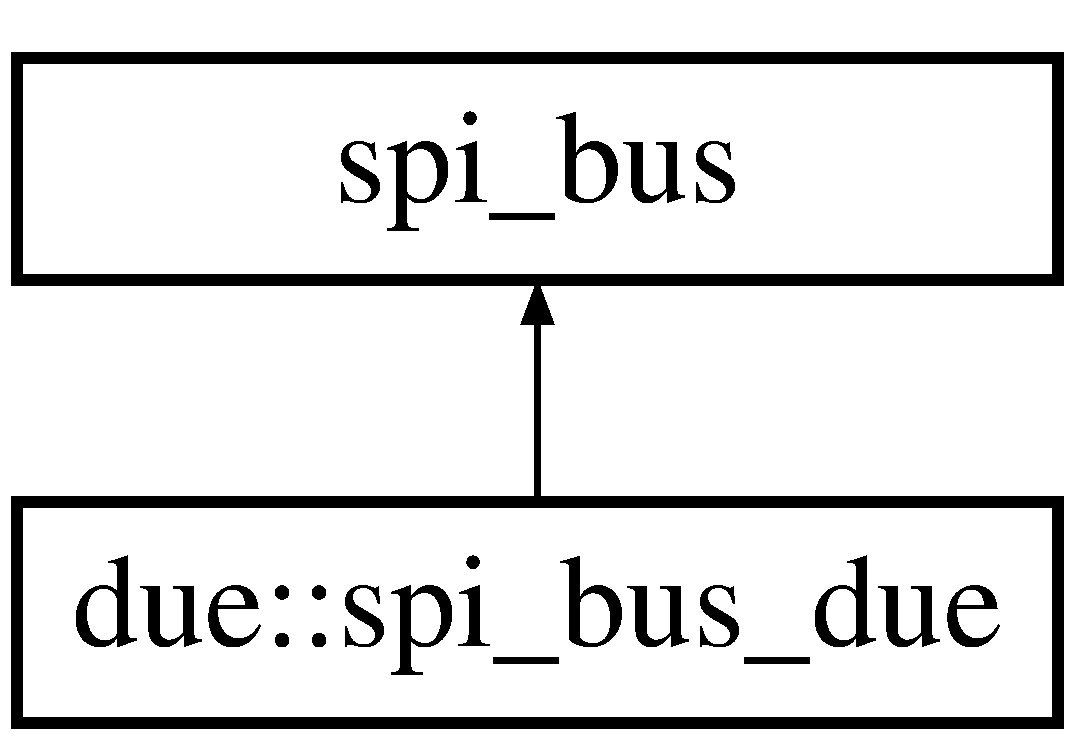
\includegraphics[height=2.000000cm]{classdue_1_1spi__bus__due}
\end{center}
\end{figure}
\subsection*{Public Member Functions}
\begin{DoxyCompactItemize}
\item 
void \hyperlink{classdue_1_1spi__bus__due_ab153084cb35b044537058d15c57a4cb8}{write\+\_\+and\+\_\+read} (hwlib\+::pin\+\_\+out \&sel, size\+\_\+t n, const uint8\+\_\+t data\+\_\+out\mbox{[}$\,$\mbox{]}, uint8\+\_\+t data\+\_\+in\mbox{[}$\,$\mbox{]}) override
\begin{DoxyCompactList}\small\item\em Write and read data. \end{DoxyCompactList}\end{DoxyCompactItemize}


\subsection{Detailed Description}
Due / sam3x8e native S\+PI bus. 

Note\+: This S\+PI class is limited to one device on the S\+PI bus. CS for the connected peripheral must be on due pin d10. 

\subsection{Member Function Documentation}
\mbox{\Hypertarget{classdue_1_1spi__bus__due_ab153084cb35b044537058d15c57a4cb8}\label{classdue_1_1spi__bus__due_ab153084cb35b044537058d15c57a4cb8}} 
\index{due\+::spi\+\_\+bus\+\_\+due@{due\+::spi\+\_\+bus\+\_\+due}!write\+\_\+and\+\_\+read@{write\+\_\+and\+\_\+read}}
\index{write\+\_\+and\+\_\+read@{write\+\_\+and\+\_\+read}!due\+::spi\+\_\+bus\+\_\+due@{due\+::spi\+\_\+bus\+\_\+due}}
\subsubsection{\texorpdfstring{write\+\_\+and\+\_\+read()}{write\_and\_read()}}
{\footnotesize\ttfamily void due\+::spi\+\_\+bus\+\_\+due\+::write\+\_\+and\+\_\+read (\begin{DoxyParamCaption}\item[{hwlib\+::pin\+\_\+out \&}]{sel,  }\item[{size\+\_\+t}]{n,  }\item[{const uint8\+\_\+t}]{data\+\_\+out\mbox{[}$\,$\mbox{]},  }\item[{uint8\+\_\+t}]{data\+\_\+in\mbox{[}$\,$\mbox{]} }\end{DoxyParamCaption})\hspace{0.3cm}{\ttfamily [inline]}, {\ttfamily [override]}}



Write and read data. 

Note\+: This request does not yield, contrary to the bitbanged S\+PI in hwlib.

\begin{DoxyWarning}{Warning}
{\ttfamily sel} is not used, CS must be on d10! 
\end{DoxyWarning}


The documentation for this class was generated from the following file\+:\begin{DoxyCompactItemize}
\item 
\hyperlink{hwlib-due-spi_8hh}{hwlib-\/due-\/spi.\+hh}\end{DoxyCompactItemize}

\chapter{File Documentation}
\hypertarget{alarm_8cc}{}\section{alarm.\+cc File Reference}
\label{alarm_8cc}\index{alarm.\+cc@{alarm.\+cc}}


The definitions of the alarm functionality of G\+A\+S-\/01.  


{\ttfamily \#include \char`\"{}alarm.\+hh\char`\"{}}\newline


\subsection{Detailed Description}
The definitions of the alarm functionality of G\+A\+S-\/01. 

\begin{DoxyAuthor}{Author}
Jeroen Kok 
\end{DoxyAuthor}
\begin{DoxyCopyright}{Copyright}
Copyright (c) 2017, The R2\+D2 Team  See L\+I\+C\+E\+N\+SE 
\end{DoxyCopyright}

\hypertarget{alarm_8hh}{}\section{alarm.\+hh File Reference}
\label{alarm_8hh}\index{alarm.\+hh@{alarm.\+hh}}


The declarations of the class \hyperlink{class_alarm}{Alarm} of G\+A\+S-\/01.  


{\ttfamily \#include \char`\"{}wrap-\/hwlib.\+hh\char`\"{}}\newline
\subsection*{Classes}
\begin{DoxyCompactItemize}
\item 
class \hyperlink{class_alarm}{Alarm}
\end{DoxyCompactItemize}


\subsection{Detailed Description}
The declarations of the class \hyperlink{class_alarm}{Alarm} of G\+A\+S-\/01. 

\begin{DoxyAuthor}{Author}
Jeroen Kok 
\end{DoxyAuthor}
\begin{DoxyCopyright}{Copyright}
Copyright (c) 2017, The R2\+D2 Team  See L\+I\+C\+E\+N\+SE 
\end{DoxyCopyright}

\hypertarget{data-logger_8cc}{}\section{C\+:/\+HU (school)/jaar2.2/(4) R2\+D2/\+R2\+D2-\/2017/modules/\+G\+A\+S/src/data-\/logger.cc File Reference}
\label{data-logger_8cc}\index{C\+:/\+H\+U (school)/jaar2.\+2/(4) R2\+D2/\+R2\+D2-\/2017/modules/\+G\+A\+S/src/data-\/logger.\+cc@{C\+:/\+H\+U (school)/jaar2.\+2/(4) R2\+D2/\+R2\+D2-\/2017/modules/\+G\+A\+S/src/data-\/logger.\+cc}}


Logs sensor data to the sd card.  


{\ttfamily \#include \char`\"{}data-\/logger.\+hh\char`\"{}}\newline


\subsection{Detailed Description}
Logs sensor data to the sd card. 

\begin{DoxyAuthor}{Author}
Paul Ettema 
\end{DoxyAuthor}
\begin{DoxyCopyright}{Copyright}
Copyright (c) 2017, The R2\+D2 Team  See L\+I\+C\+E\+N\+SE 
\end{DoxyCopyright}

\hypertarget{data-logger_8hh}{}\section{data-\/logger.hh File Reference}
\label{data-logger_8hh}\index{data-\/logger.\+hh@{data-\/logger.\+hh}}


Logs sensor data to the sd card.  


{\ttfamily \#include \char`\"{}sd-\/spi.\+hh\char`\"{}}\newline
\subsection*{Classes}
\begin{DoxyCompactItemize}
\item 
class \hyperlink{class_data_logger}{Data\+Logger}
\end{DoxyCompactItemize}


\subsection{Detailed Description}
Logs sensor data to the sd card. 

\begin{DoxyAuthor}{Author}
Paul Ettema 
\end{DoxyAuthor}
\begin{DoxyCopyright}{Copyright}
Copyright (c) 2017, The R2\+D2 Team  See L\+I\+C\+E\+N\+SE 
\end{DoxyCopyright}

\hypertarget{hwlib-due-spi_8hh}{}\section{hwlib-\/due-\/spi.hh File Reference}
\label{hwlib-due-spi_8hh}\index{hwlib-\/due-\/spi.\+hh@{hwlib-\/due-\/spi.\+hh}}


Due / sam3x8e native S\+PI.  


{\ttfamily \#include \char`\"{}wrap-\/hwlib.\+hh\char`\"{}}\newline
\subsection*{Classes}
\begin{DoxyCompactItemize}
\item 
class \hyperlink{classdue_1_1spi__bus__due}{due\+::spi\+\_\+bus\+\_\+due}
\begin{DoxyCompactList}\small\item\em Due / sam3x8e native S\+PI bus. \end{DoxyCompactList}\end{DoxyCompactItemize}
\subsection*{Functions}
\begin{DoxyCompactItemize}
\item 
\mbox{\Hypertarget{hwlib-due-spi_8hh_af52720fcb38ebf98b8dcf75b1bfc8188}\label{hwlib-due-spi_8hh_af52720fcb38ebf98b8dcf75b1bfc8188}} 
constexpr uint32\+\_\+t {\bfseries due\+::\+S\+P\+I\+\_\+\+P\+CS} (uint32\+\_\+t npcs)
\end{DoxyCompactItemize}


\subsection{Detailed Description}
Due / sam3x8e native S\+PI. 

\begin{DoxyAuthor}{Author}
Chris Smeele 
\end{DoxyAuthor}
\begin{DoxyDate}{Date}
2016-\/10-\/09 
\end{DoxyDate}
\begin{DoxyCopyright}{Copyright}
Copyright (c) 2016, Chris Smeele
\end{DoxyCopyright}
Distributed under the Boost Software License, Version 1.\+0. (See accompanying file L\+I\+C\+E\+N\+S\+E\+\_\+1\+\_\+0.\+txt or copy at \href{http://www.boost.org/LICENSE_1_0.txt}{\tt http\+://www.\+boost.\+org/\+L\+I\+C\+E\+N\+S\+E\+\_\+1\+\_\+0.\+txt}) 
\hypertarget{libc-stub_8cc}{}\section{C\+:/\+HU (school)/jaar2.2/(4) R2\+D2/\+R2\+D2-\/2017/modules/\+G\+A\+S/src/libc-\/stub.cc File Reference}
\label{libc-stub_8cc}\index{C\+:/\+H\+U (school)/jaar2.\+2/(4) R2\+D2/\+R2\+D2-\/2017/modules/\+G\+A\+S/src/libc-\/stub.\+cc@{C\+:/\+H\+U (school)/jaar2.\+2/(4) R2\+D2/\+R2\+D2-\/2017/modules/\+G\+A\+S/src/libc-\/stub.\+cc}}


Libc stub code.  


\subsection*{Typedefs}
\begin{DoxyCompactItemize}
\item 
\mbox{\Hypertarget{libc-stub_8cc_afadb78ab5a0fd50f0607f9bc7ae0235a}\label{libc-stub_8cc_afadb78ab5a0fd50f0607f9bc7ae0235a}} 
using {\bfseries size\+\_\+t} = unsigned int
\end{DoxyCompactItemize}
\subsection*{Functions}
\begin{DoxyCompactItemize}
\item 
\mbox{\Hypertarget{libc-stub_8cc_a5227870c8dd60cda7add3fa24aa00a7b}\label{libc-stub_8cc_a5227870c8dd60cda7add3fa24aa00a7b}} 
void {\bfseries \+\_\+\+\_\+libc\+\_\+init\+\_\+array} ()
\item 
\mbox{\Hypertarget{libc-stub_8cc_a9d9bc4578fa6ef77862846c794b3bcc0}\label{libc-stub_8cc_a9d9bc4578fa6ef77862846c794b3bcc0}} 
void $\ast$ {\bfseries memset} (void $\ast$m, int v, size\+\_\+t size)
\item 
\mbox{\Hypertarget{libc-stub_8cc_a221995d01087b6da7d0df8d004c7797b}\label{libc-stub_8cc_a221995d01087b6da7d0df8d004c7797b}} 
void $\ast$ {\bfseries memcpy} (void $\ast$dst, const void $\ast$src, size\+\_\+t size)
\item 
\mbox{\Hypertarget{libc-stub_8cc_a6f9d2861931acb9dad897ad7a62eb23f}\label{libc-stub_8cc_a6f9d2861931acb9dad897ad7a62eb23f}} 
void {\bfseries operator delete} (void $\ast$p, size\+\_\+t x)  throw ()
\item 
\mbox{\Hypertarget{libc-stub_8cc_a86107594327f3a001230df9802cd4422}\label{libc-stub_8cc_a86107594327f3a001230df9802cd4422}} 
void {\bfseries operator delete} (void $\ast$p)  throw ()
\end{DoxyCompactItemize}


\subsection{Detailed Description}
Libc stub code. 

\begin{DoxyAuthor}{Author}
Chris Smeele 
\end{DoxyAuthor}
\begin{DoxyCopyright}{Copyright}
Copyright (c) 2017, The R2\+D2 Team  See L\+I\+C\+E\+N\+SE 
\end{DoxyCopyright}

\hypertarget{main_8cc}{}\section{C\+:/\+HU (school)/jaar2.2/(4) R2\+D2/\+R2\+D2-\/2017/modules/\+G\+A\+S/src/main.cc File Reference}
\label{main_8cc}\index{C\+:/\+H\+U (school)/jaar2.\+2/(4) R2\+D2/\+R2\+D2-\/2017/modules/\+G\+A\+S/src/main.\+cc@{C\+:/\+H\+U (school)/jaar2.\+2/(4) R2\+D2/\+R2\+D2-\/2017/modules/\+G\+A\+S/src/main.\+cc}}


G\+AS module main.  


{\ttfamily \#include \char`\"{}wrap-\/hwlib.\+hh\char`\"{}}\newline
{\ttfamily \#include \char`\"{}hwlib-\/due-\/spi.\+hh\char`\"{}}\newline
{\ttfamily \#include \char`\"{}sd-\/spi.\+hh\char`\"{}}\newline
{\ttfamily \#include \char`\"{}data-\/logger.\+hh\char`\"{}}\newline
{\ttfamily \#include \char`\"{}alarm.\+hh\char`\"{}}\newline
\subsection*{Functions}
\begin{DoxyCompactItemize}
\item 
float \hyperlink{main_8cc_a0c36c174a506e50bfe004be1f70b19d4}{read\+Gas\+Sensor} (hwlib\+::target\+::pin\+\_\+adc \&sensor)
\begin{DoxyCompactList}\small\item\em Reads the gas sensor data. \end{DoxyCompactList}\item 
\mbox{\Hypertarget{main_8cc_ae66f6b31b5ad750f1fe042a706a4e3d4}\label{main_8cc_ae66f6b31b5ad750f1fe042a706a4e3d4}} 
int {\bfseries main} ()
\end{DoxyCompactItemize}


\subsection{Detailed Description}
G\+AS module main. 

\begin{DoxyAuthor}{Author}
Chris Smeele 

David Driessen 

Paul Ettema 
\end{DoxyAuthor}
\begin{DoxyCopyright}{Copyright}
Copyright (c) 2017, The R2\+D2 Team  See L\+I\+C\+E\+N\+SE 
\end{DoxyCopyright}


\subsection{Function Documentation}
\mbox{\Hypertarget{main_8cc_a0c36c174a506e50bfe004be1f70b19d4}\label{main_8cc_a0c36c174a506e50bfe004be1f70b19d4}} 
\index{main.\+cc@{main.\+cc}!read\+Gas\+Sensor@{read\+Gas\+Sensor}}
\index{read\+Gas\+Sensor@{read\+Gas\+Sensor}!main.\+cc@{main.\+cc}}
\subsubsection{\texorpdfstring{read\+Gas\+Sensor()}{readGasSensor()}}
{\footnotesize\ttfamily float read\+Gas\+Sensor (\begin{DoxyParamCaption}\item[{hwlib\+::target\+::pin\+\_\+adc \&}]{sensor }\end{DoxyParamCaption})}



Reads the gas sensor data. 


\begin{DoxyParams}{Parameters}
{\em sensor} & The analog pin the gas sensor is connected to \\
\hline
\end{DoxyParams}
\begin{DoxyReturn}{Returns}
The measured data as float voltage 
\end{DoxyReturn}

\hypertarget{sd-spi_8cc}{}\section{C\+:/\+HU (school)/jaar2.2/(4) R2\+D2/\+R2\+D2-\/2017/modules/\+G\+A\+S/src/sd-\/spi.cc File Reference}
\label{sd-spi_8cc}\index{C\+:/\+H\+U (school)/jaar2.\+2/(4) R2\+D2/\+R2\+D2-\/2017/modules/\+G\+A\+S/src/sd-\/spi.\+cc@{C\+:/\+H\+U (school)/jaar2.\+2/(4) R2\+D2/\+R2\+D2-\/2017/modules/\+G\+A\+S/src/sd-\/spi.\+cc}}


SD S\+PI Store provider.  


{\ttfamily \#include \char`\"{}sd-\/spi.\+hh\char`\"{}}\newline
{\ttfamily \#include $<$cstdlib$>$}\newline
{\ttfamily \#include $<$cstring$>$}\newline
{\ttfamily \#include $<$cmath$>$}\newline
\subsection*{Classes}
\begin{DoxyCompactItemize}
\item 
struct \hyperlink{struct_sd_csd}{Sd\+Csd}
\begin{DoxyCompactList}\small\item\em SD Card-\/\+Specific Data structure. \end{DoxyCompactList}\end{DoxyCompactItemize}
\subsection*{Functions}
\begin{DoxyCompactItemize}
\item 
\mbox{\Hypertarget{sd-spi_8cc_a65cc01dcd598989a32314bc110f023c6}\label{sd-spi_8cc_a65cc01dcd598989a32314bc110f023c6}} 
struct \hyperlink{struct_sd_csd}{Sd\+Csd} {\bfseries \+\_\+\+\_\+attribute\+\_\+\+\_\+} ((packed))
\end{DoxyCompactItemize}
\subsection*{Variables}
\begin{DoxyCompactItemize}
\item 
\mbox{\Hypertarget{sd-spi_8cc_ab22abc2906422da61885ac6c8e6a1a59}\label{sd-spi_8cc_ab22abc2906422da61885ac6c8e6a1a59}} 
uint8\+\_\+t {\bfseries version}
\item 
\mbox{\Hypertarget{sd-spi_8cc_aacf668a96bedab028a9e5e0be7b6a464}\label{sd-spi_8cc_aacf668a96bedab028a9e5e0be7b6a464}} 
uint8\+\_\+t {\bfseries \+\_\+reserved1}
\item 
\mbox{\Hypertarget{sd-spi_8cc_a0966d27ae7950edf851c154da1bc0183}\label{sd-spi_8cc_a0966d27ae7950edf851c154da1bc0183}} 
uint8\+\_\+t {\bfseries taac}
\item 
\mbox{\Hypertarget{sd-spi_8cc_aade95f8dc286c76838b3996c03446642}\label{sd-spi_8cc_aade95f8dc286c76838b3996c03446642}} 
uint8\+\_\+t {\bfseries nsac}
\item 
\mbox{\Hypertarget{sd-spi_8cc_a4b6a2939dcf7ce0651cf15c6731a942e}\label{sd-spi_8cc_a4b6a2939dcf7ce0651cf15c6731a942e}} 
uint8\+\_\+t {\bfseries tran\+Speed}
\item 
\mbox{\Hypertarget{sd-spi_8cc_a92ee6c5b58356ffb18b92f37002650bd}\label{sd-spi_8cc_a92ee6c5b58356ffb18b92f37002650bd}} 
uint16\+\_\+t {\bfseries ccc}
\item 
\mbox{\Hypertarget{sd-spi_8cc_a25f4bd4d6487054f36dd9c66dcf4b88c}\label{sd-spi_8cc_a25f4bd4d6487054f36dd9c66dcf4b88c}} 
uint8\+\_\+t {\bfseries read\+Bl\+Len}
\item 
\mbox{\Hypertarget{sd-spi_8cc_a68ff61f034e693a8cbdca66969c06693}\label{sd-spi_8cc_a68ff61f034e693a8cbdca66969c06693}} 
uint8\+\_\+t {\bfseries read\+Bl\+Partial}
\item 
\mbox{\Hypertarget{sd-spi_8cc_aae4029e5691d7fa675e9d37913546c14}\label{sd-spi_8cc_aae4029e5691d7fa675e9d37913546c14}} 
uint8\+\_\+t {\bfseries write\+Blk\+Misalign}
\item 
\mbox{\Hypertarget{sd-spi_8cc_ae0b87455c929aad1229160b974217d50}\label{sd-spi_8cc_ae0b87455c929aad1229160b974217d50}} 
uint8\+\_\+t {\bfseries read\+Blk\+Misalign}
\item 
\mbox{\Hypertarget{sd-spi_8cc_a11e1a7cd80607df9c541b9b93fdcdd71}\label{sd-spi_8cc_a11e1a7cd80607df9c541b9b93fdcdd71}} 
uint8\+\_\+t {\bfseries dsr\+Imp}
\item 
\mbox{\Hypertarget{sd-spi_8cc_aa5560a50b81a8fec9949a071aa5692c3}\label{sd-spi_8cc_aa5560a50b81a8fec9949a071aa5692c3}} 
uint8\+\_\+t {\bfseries \+\_\+reserved2}
\item 
\mbox{\Hypertarget{sd-spi_8cc_a18e891c55aa5c118eb322064bcf2b6f2}\label{sd-spi_8cc_a18e891c55aa5c118eb322064bcf2b6f2}} 
uint32\+\_\+t {\bfseries c\+Size}
\item 
\mbox{\Hypertarget{sd-spi_8cc_a138402c40e50631272b95f65ed3367fd}\label{sd-spi_8cc_a138402c40e50631272b95f65ed3367fd}} 
uint8\+\_\+t {\bfseries \+\_\+reserved3}
\item 
\mbox{\Hypertarget{sd-spi_8cc_ac85bfdbd98595d83c4c2dc9e52f7d2b5}\label{sd-spi_8cc_ac85bfdbd98595d83c4c2dc9e52f7d2b5}} 
uint8\+\_\+t {\bfseries erase\+Blk\+En}
\item 
\mbox{\Hypertarget{sd-spi_8cc_a1f111c9e911c19b2f2f4e570f3109a8a}\label{sd-spi_8cc_a1f111c9e911c19b2f2f4e570f3109a8a}} 
uint8\+\_\+t {\bfseries sector\+Size}
\item 
\mbox{\Hypertarget{sd-spi_8cc_a4fecdd0b83dee23b02b2a33feb336525}\label{sd-spi_8cc_a4fecdd0b83dee23b02b2a33feb336525}} 
uint8\+\_\+t {\bfseries wp\+Grp\+Size}
\item 
\mbox{\Hypertarget{sd-spi_8cc_ae277594f3bf506837915af23cf62538b}\label{sd-spi_8cc_ae277594f3bf506837915af23cf62538b}} 
uint8\+\_\+t {\bfseries wp\+Grp\+Enable}
\item 
\mbox{\Hypertarget{sd-spi_8cc_ac9746ab436933fee44b77ec24bab5246}\label{sd-spi_8cc_ac9746ab436933fee44b77ec24bab5246}} 
uint8\+\_\+t {\bfseries \+\_\+reserved4}
\item 
\mbox{\Hypertarget{sd-spi_8cc_a502def73625d1c01a6d073c948bbbddf}\label{sd-spi_8cc_a502def73625d1c01a6d073c948bbbddf}} 
uint8\+\_\+t {\bfseries r2w\+Factor}
\item 
\mbox{\Hypertarget{sd-spi_8cc_a4dc0443fc7da9c551afa5c3b7ff5a9a2}\label{sd-spi_8cc_a4dc0443fc7da9c551afa5c3b7ff5a9a2}} 
uint8\+\_\+t {\bfseries write\+Bl\+Len}
\item 
\mbox{\Hypertarget{sd-spi_8cc_ab90538206d784d55eccda7439b51c3ff}\label{sd-spi_8cc_ab90538206d784d55eccda7439b51c3ff}} 
uint8\+\_\+t {\bfseries write\+Bl\+Partial}
\item 
\mbox{\Hypertarget{sd-spi_8cc_a9466da9396b5ca62e38aa350c85695e3}\label{sd-spi_8cc_a9466da9396b5ca62e38aa350c85695e3}} 
uint8\+\_\+t {\bfseries \+\_\+reserved5}
\item 
\mbox{\Hypertarget{sd-spi_8cc_a7d1a7971343dec51da77f1f8f190095d}\label{sd-spi_8cc_a7d1a7971343dec51da77f1f8f190095d}} 
uint8\+\_\+t {\bfseries file\+Format\+Grp}
\item 
\mbox{\Hypertarget{sd-spi_8cc_a67fee7b8c9aec8b858b32efda2e943ed}\label{sd-spi_8cc_a67fee7b8c9aec8b858b32efda2e943ed}} 
uint8\+\_\+t {\bfseries copy}
\item 
\mbox{\Hypertarget{sd-spi_8cc_abd25a030c5ca3c66cbd548cd1ee0ab4f}\label{sd-spi_8cc_abd25a030c5ca3c66cbd548cd1ee0ab4f}} 
uint8\+\_\+t {\bfseries perm\+Write\+Protect}
\item 
\mbox{\Hypertarget{sd-spi_8cc_a26aaca9a408a293c2c021701199a686c}\label{sd-spi_8cc_a26aaca9a408a293c2c021701199a686c}} 
uint8\+\_\+t {\bfseries tmp\+Write\+Protect}
\item 
\mbox{\Hypertarget{sd-spi_8cc_afa318ea025b4c0f3078220051cb34222}\label{sd-spi_8cc_afa318ea025b4c0f3078220051cb34222}} 
uint8\+\_\+t {\bfseries file\+Format}
\item 
\mbox{\Hypertarget{sd-spi_8cc_a3bd4f1524a863a283ab87cddd99e1935}\label{sd-spi_8cc_a3bd4f1524a863a283ab87cddd99e1935}} 
uint8\+\_\+t {\bfseries \+\_\+reserved6}
\item 
\mbox{\Hypertarget{sd-spi_8cc_a2bb48654c986c72b5979b9be82ad5fbc}\label{sd-spi_8cc_a2bb48654c986c72b5979b9be82ad5fbc}} 
uint8\+\_\+t {\bfseries crc7}
\item 
\mbox{\Hypertarget{sd-spi_8cc_aa3665e83385c8c805aa543bf16ee1528}\label{sd-spi_8cc_aa3665e83385c8c805aa543bf16ee1528}} 
uint8\+\_\+t {\bfseries \+\_\+end\+Bit}
\end{DoxyCompactItemize}


\subsection{Detailed Description}
SD S\+PI Store provider. 

\begin{DoxyAuthor}{Author}
Chris Smeele 

Paul Ettema 
\end{DoxyAuthor}
\begin{DoxyCopyright}{Copyright}
Copyright (c) 2017, The R2\+D2 Team  See L\+I\+C\+E\+N\+SE
\end{DoxyCopyright}
SD S\+PI Store provider from \href{https://github.com/cjsmeele/Picus}{\tt https\+://github.\+com/cjsmeele/\+Picus} ported to use hwlib and work inside the R2\+D2 Project by Paul Ettema

Original file is copyright 2016 (c) Chris Smeele and licensed under G\+P\+Lv3. This file is modified and relicensed under the Apache license with the original author\textquotesingle{}s permission. 
\hypertarget{sd-spi_8hh}{}\section{C\+:/\+HU (school)/jaar2.2/(4) R2\+D2/\+R2\+D2-\/2017/modules/\+G\+A\+S/src/sd-\/spi.hh File Reference}
\label{sd-spi_8hh}\index{C\+:/\+H\+U (school)/jaar2.\+2/(4) R2\+D2/\+R2\+D2-\/2017/modules/\+G\+A\+S/src/sd-\/spi.\+hh@{C\+:/\+H\+U (school)/jaar2.\+2/(4) R2\+D2/\+R2\+D2-\/2017/modules/\+G\+A\+S/src/sd-\/spi.\+hh}}


SD S\+PI Store provider.  


{\ttfamily \#include \char`\"{}wrap-\/hwlib.\+hh\char`\"{}}\newline
{\ttfamily \#include $<$store.\+hh$>$}\newline
\subsection*{Classes}
\begin{DoxyCompactItemize}
\item 
class \hyperlink{class_sd_spi}{Sd\+Spi}
\begin{DoxyCompactList}\small\item\em Provides a SD S\+PI Block Storage Provider. \end{DoxyCompactList}\end{DoxyCompactItemize}
\subsection*{Variables}
\begin{DoxyCompactItemize}
\item 
\mbox{\Hypertarget{sd-spi_8hh_ac74ade0daa8170c6112d3540d621e598}\label{sd-spi_8hh_ac74ade0daa8170c6112d3540d621e598}} 
\hyperlink{class_sd_spi}{Sd\+Spi} {\bfseries \+\_\+\+\_\+attribute\+\_\+\+\_\+}
\end{DoxyCompactItemize}


\subsection{Detailed Description}
SD S\+PI Store provider. 

\begin{DoxyAuthor}{Author}
Chris Smeele 

Paul Ettema 
\end{DoxyAuthor}
\begin{DoxyCopyright}{Copyright}
Copyright (c) 2017, The R2\+D2 Team  See L\+I\+C\+E\+N\+SE SD S\+PI Store provider from \href{https://github.com/cjsmeele/Picus}{\tt https\+://github.\+com/cjsmeele/\+Picus} ported to use hwlib and work inside the R2\+D2 Project by Paul Ettema
\end{DoxyCopyright}
Original file is copyright 2016 (c) Chris Smeele and licensed under G\+P\+Lv3. This file is modified and relicensed under the Apache license with the original author\textquotesingle{}s permission. 
%--- End generated contents ---

% Index
\backmatter
\newpage
\phantomsection
\clearemptydoublepage
\addcontentsline{toc}{chapter}{Index}
\printindex

\end{document}
